\section{Implementation}
To combine SLP with our group key agreement protocol we changed/added following protocol properties:
\begin{itemize}
  \item SLP message
  \item Message integrity
  \item Key exchange
  \item Communication
\end{itemize}

\subsection{SecuredSLP message format}
The header of a SLP message was modified to distinguish SLP messages from SecuredSLP messages. We added the \texttt{S}, \texttt{Security Group Length} and \texttt{Security Group Name} flags into the header and changed the \texttt{Version} of SLP in the source code (compare figures \ref{fig:slp-header} and \ref{fig:sslp-header}).
\begin{description}
\item[Version:] Is now set to 3.
\item[S:] This flag shows that the message body is encrypted.
\item[Security Group Length:] This flag specifies the length of the \texttt{Security Group Name} string.  
\item[Securety Group Name:] This flag shows the name of the security group the message belongs to.
\end{description}
\texttt{Security Group Length} and \texttt{Security Group Name} are both key identifier. Those are used to decide with which group share key the message should be decrypted. This two flags are analog to the SPI (Secure Parameter Index) in SLPv2. In SecuredSLP we call them SGPI (Secure Group Parameter Index).
\begin{figure}[!h]
\begin{lstlisting}
	 0                   1                   2                   3
	 0 1 2 3 4 5 6 7 8 9 0 1 2 3 4 5 6 7 8 9 0 1 2 3 4 5 6 7 8 9 0 1
	+-+-+-+-+-+-+-+-+-+-+-+-+-+-+-+-+-+-+-+-+-+-+-+-+-+-+-+-+-+-+-+-+
	|    Version    |  Function-ID  |            Length             |
	+-+-+-+-+-+-+-+-+-+-+-+-+-+-+-+-+-+-+-+-+-+-+-+-+-+-+-+-+-+-+-+-+
	| Length, contd.|O|F|R|       reserved          |Next Ext Offset|
	+-+-+-+-+-+-+-+-+-+-+-+-+-+-+-+-+-+-+-+-+-+-+-+-+-+-+-+-+-+-+-+-+
	| Next Extension Offset, contd. |              XID              |
	+-+-+-+-+-+-+-+-+-+-+-+-+-+-+-+-+-+-+-+-+-+-+-+-+-+-+-+-+-+-+-+-+
	|      Language Tag Length      |         Language Tag          |
	+-+-+-+-+-+-+-+-+-+-+-+-+-+-+-+-+-+-+-+-+-+-+-+-+-+-+-+-+-+-+-+-+
\end{lstlisting}
\caption{SLPv2 Header}
\label{fig:slp-header}
\end{figure}

\begin{figure}[!h]
\begin{lstlisting}
	 0                   1                   2                   3
	 0 1 2 3 4 5 6 7 8 9 0 1 2 3 4 5 6 7 8 9 0 1 2 3 4 5 6 7 8 9 0 1
	+-+-+-+-+-+-+-+-+-+-+-+-+-+-+-+-+-+-+-+-+-+-+-+-+-+-+-+-+-+-+-+-+
	|    Version    |  Function-ID  |            Length             |
	+-+-+-+-+-+-+-+-+-+-+-+-+-+-+-+-+-+-+-+-+-+-+-+-+-+-+-+-+-+-+-+-+
	| Length, contd.|O|F|R|S|     reserved          |Next Ext Offset|
	+-+-+-+-+-+-+-+-+-+-+-+-+-+-+-+-+-+-+-+-+-+-+-+-+-+-+-+-+-+-+-+-+
	| Next Extension Offset, contd. |              XID              |
	+-+-+-+-+-+-+-+-+-+-+-+-+-+-+-+-+-+-+-+-+-+-+-+-+-+-+-+-+-+-+-+-+
	|      Language Tag Length      |         Language Tag          |
	+-+-+-+-+-+-+-+-+-+-+-+-+-+-+-+-+-+-+-+-+-+-+-+-+-+-+-+-+-+-+-+-+
	|     Security Group Length     |      Security Group Name      |
	+-+-+-+-+-+-+-+-+-+-+-+-+-+-+-+-+-+-+-+-+-+-+-+-+-+-+-+-+-+-+-+-+
\end{lstlisting}
\caption{SecuredSLP Header}
\label{fig:sslp-header}
\end{figure}

\subsubsection{Message integrity}
Additionally we need to ensure the message integrity to prevent several attacks. Otherwise it would be possible for example to change the XID of a message to reply on a not matching ServiceRequest or run a replay attack on ServiceReply for services which not exist anymore. To solve such problems we use a HMAC (96 Bit) over the header and the encrypted message body so the header and payload are linked with each other (\cite{Kraw97} and \cite{Kero00}). This method is also used in IPSec under the ESP mode and allows us to prevent replay attacks and header manipulation of each SecuredSLP message. See also section \ref{sub:Replay-Prevention}. The whole SecuredSLP message is shown in figure \ref{fig:sslp-message}.
\begin{figure}[!h]
\centering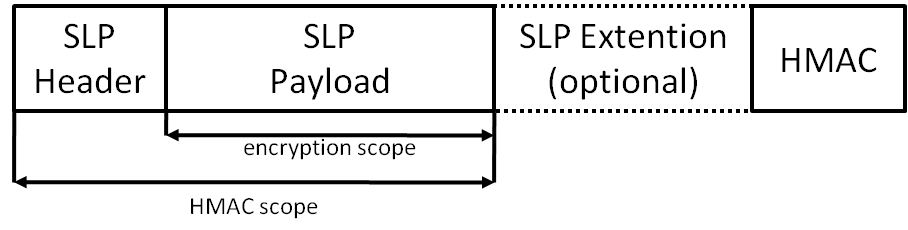
\includegraphics[width=0.5\textwidth]{Images/HMAC}
\caption{SecuredSLP message}
\label{fig:sslp-message}
\end{figure}


\subsection{Key exchange in SecuredSLP}\label{sec:keyexchange}
Like discussed above we use a group key agreement protocol to establish security between group members. To get knowledge about a security group, clients use extra discovery iteration. The information about a security group is announced as plain text; otherwise no one would be able to get knowledge about such a group. To join a security group a user has to send a join message to the group. Then the group key agreement protocol handles the key distribution. In our implementation we used TGDH, so the distribution works like discussed in section \ref{sec:TGDH}. After receiving the group key, security group members are able to discover services which are announced in this security group or provide services themselves. Also there is a rekeying phase after a user leaves the group. That is important to keep the security under the group members and to avoid that a key gets compromised. The key exchange doesn't increase the performance of SLP but raises the security aspects discussed in section \ref{sec:conclusion}.

\subsection{Communication in SecuredSLP}
Due to the additional changes in the protocol it is necessary to take a look at the communication between network members. SecuredSLP still provides unencrypted communication like in SLPv2 so it is still possible to create or join an unsafe SLP scope. In that case the communication works like in SLPv2 (compare section \ref{sec:intro}) without a group agreement protocol. In case SecuredSLP tries to establish connection to a security group the communication can be described as following:
\begin{figure}[!h]
\centering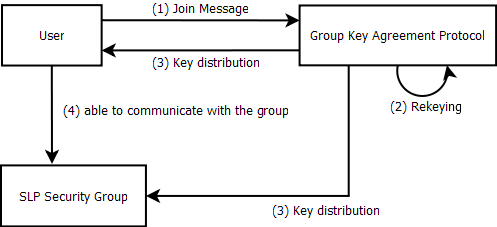
\includegraphics[width=0.5\textwidth]{Images/sSLP_join}
\caption{Communication sequence of a user joining a SecuredSLP security group}
\label{fig:sslp_join}
\end{figure}
\begin{enumerate}
  \item User discovers a security group and uses the interface of the group agreement protocol to get access to the security group.
  \item Group key agreement protocol initializes the rekeying phase and computes new group key.
  \item Group key agreement protocol distributes the new group key to the old security group members and to the new member, so the security group members are able to communicate with each other. Compare with figure \ref{fig:sslp_join}.
\end{enumerate}
Like told above the group agreement protocol is just a module adjacent to SLP and works asynchronous with it. Hence the key distribution is more complicated and fault-prone. Also there is just one valid key in the network at time so most problems arrive if a rekeying phase is initialized and there are still messages in the network encrypted with the old group key. Those messages will be refused by SecuredSLP.\\\\
\textcolor{red}{---------Sequenzdiagramm erkl�ren---------}\\
After joining a group security group member are able to advertise and discover services like depict in figure \ref{fig:SequenceDiagramm}.
\begin{enumerate}[label=\arabic{*}:]
  \item SA wants to announce a service with a specified object and a KeyPair.
  \item New security group is initialized, an already existing group is used, respectively.
  \item Service is announced via multicast to the whole security group.
  \item \textcolor{red}{nochmal?}
  \item UA wants to discover services
\end{enumerate}
\textcolor{red}{---------Sequenzdiagramm erkl�ren---------}
\begin{figure*}[!h]
\centering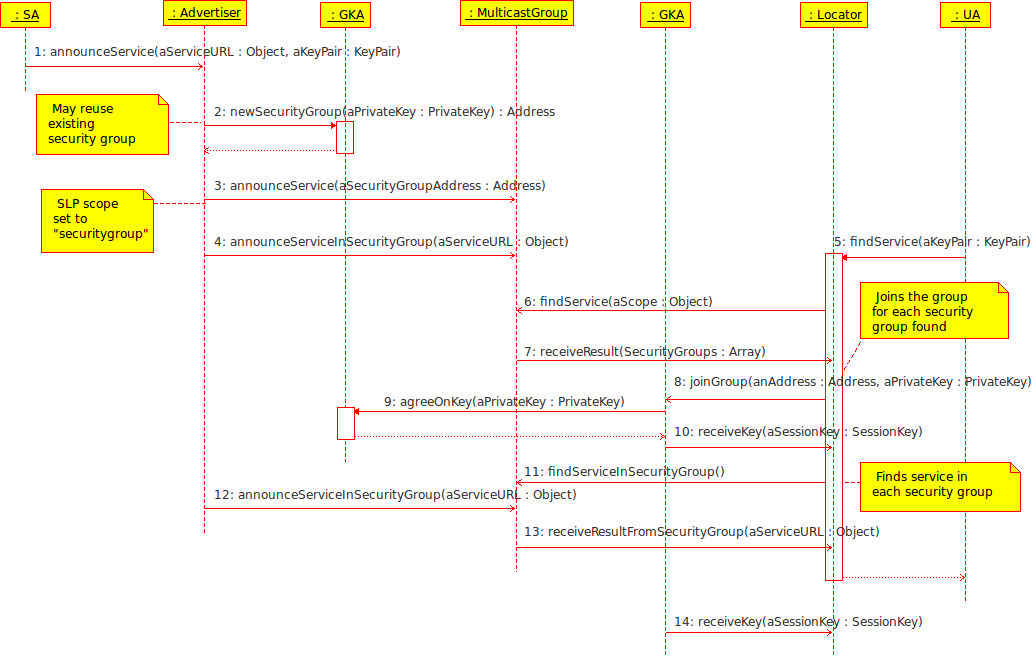
\includegraphics[width=1.0\textwidth]{Images/SequenceDiagramm}
\caption{Sequence diagramm of service announcement and service discovery in SecuredSLP}
\label{fig:SequenceDiagramm}
\end{figure*}